\documentclass{standalone}
\usepackage{tikz}
\usetikzlibrary{patterns, positioning}
\usepackage[sfdefault]{ClearSans} %% option 'sfdefault' activates Clear Sans as the default text font
\usepackage[T1]{fontenc}

\begin{document}
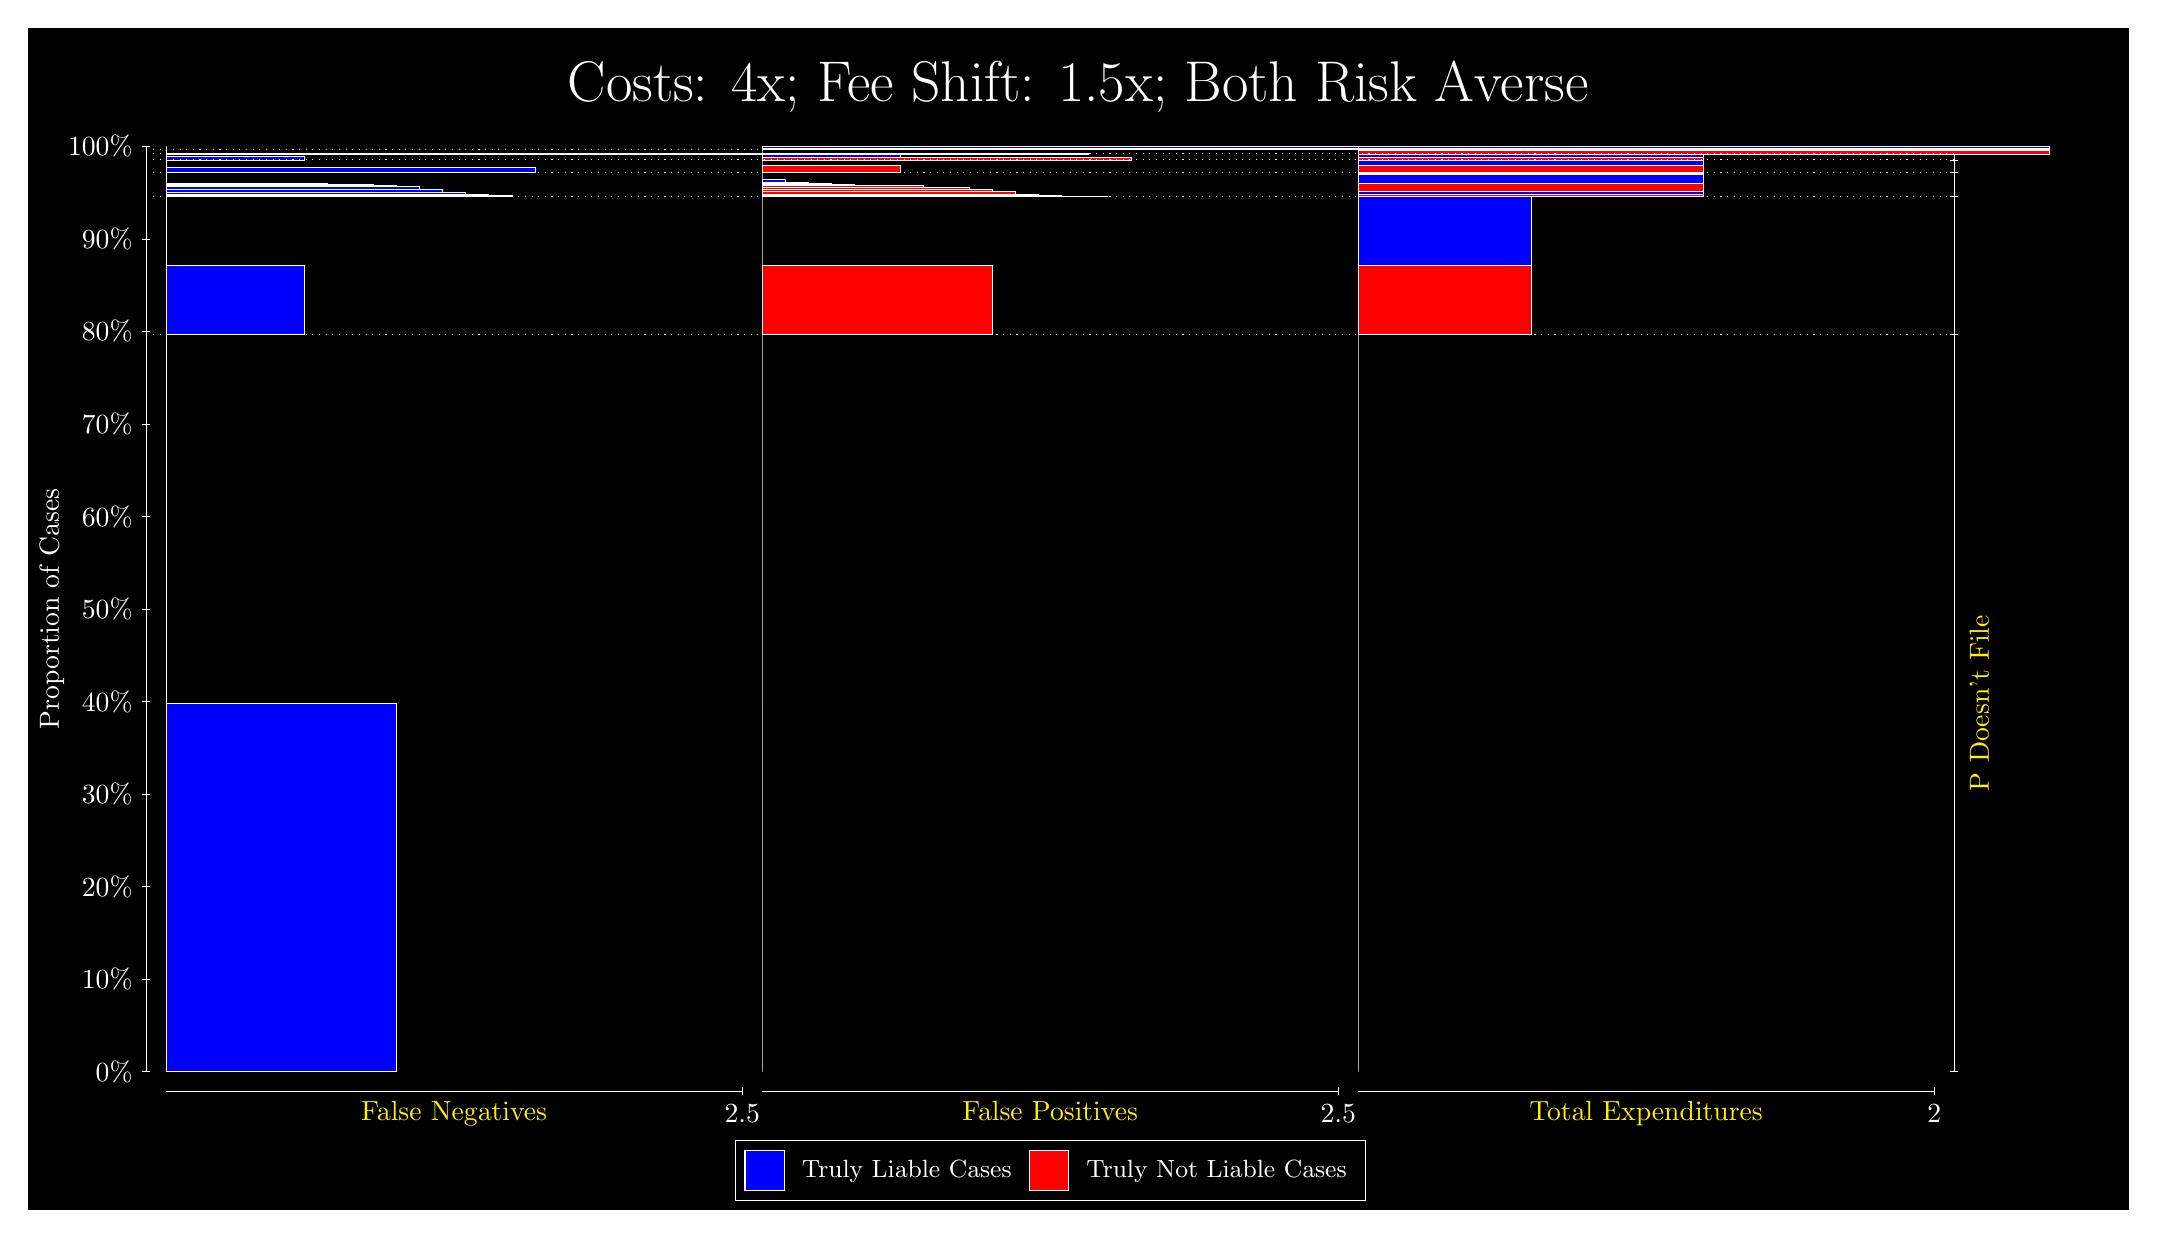
\begin{tikzpicture}
\draw[fill=black] (0,0) rectangle (26.667,15);
\draw[text=white] (0,13.5) rectangle (26.667,15) node[midway] {\huge Costs: 4x; Fee Shift: 1.5x; Both Risk Averse};
\draw[white, very thin] (1.5,1.75) -- (1.5,13.5);
\node[rotate=90, text=white, anchor=center] at (0.3, 7.625) {Proportion of Cases};
\draw[white, very thin] (1.45,1.75) -- (1.55,1.75);
\node[text=white, anchor=east] at (1.45, 1.75) {0\%};
\draw[white, very thin] (1.45,2.925) -- (1.55,2.925);
\node[text=white, anchor=east] at (1.45, 2.925) {10\%};
\draw[white, very thin] (1.45,4.1) -- (1.55,4.1);
\node[text=white, anchor=east] at (1.45, 4.1) {20\%};
\draw[white, very thin] (1.45,5.275) -- (1.55,5.275);
\node[text=white, anchor=east] at (1.45, 5.275) {30\%};
\draw[white, very thin] (1.45,6.45) -- (1.55,6.45);
\node[text=white, anchor=east] at (1.45, 6.45) {40\%};
\draw[white, very thin] (1.45,7.625) -- (1.55,7.625);
\node[text=white, anchor=east] at (1.45, 7.625) {50\%};
\draw[white, very thin] (1.45,8.8) -- (1.55,8.8);
\node[text=white, anchor=east] at (1.45, 8.8) {60\%};
\draw[white, very thin] (1.45,9.975) -- (1.55,9.975);
\node[text=white, anchor=east] at (1.45, 9.975) {70\%};
\draw[white, very thin] (1.45,11.15) -- (1.55,11.15);
\node[text=white, anchor=east] at (1.45, 11.15) {80\%};
\draw[white, very thin] (1.45,12.325) -- (1.55,12.325);
\node[text=white, anchor=east] at (1.45, 12.325) {90\%};
\draw[white, very thin] (1.45,13.5) -- (1.55,13.5);
\node[text=white, anchor=east] at (1.45, 13.5) {100\%};

\draw[white, very thin] (24.457,1.75) -- (24.457,13.5);
\draw[white, very thin] (24.407,1.75) -- (24.507,1.75);
\node[anchor=west] at (24.407, 1.75) {};
\draw[white, very thin] (24.407,11.108) -- (24.507,11.108);
\node[anchor=west] at (24.407, 11.108) {};
\draw[white, very thin] (24.407,12.862) -- (24.507,12.862);
\node[anchor=west] at (24.407, 12.862) {};
\draw[white, very thin] (24.407,13.169) -- (24.507,13.169);
\node[anchor=west] at (24.407, 13.169) {};
\draw[white, very thin] (24.407,13.328) -- (24.507,13.328);
\node[anchor=west] at (24.407, 13.328) {};
\draw[white, very thin] (24.407,13.404) -- (24.507,13.404);
\node[anchor=west] at (24.407, 13.404) {};
\draw[white, very thin] (24.407,13.46) -- (24.507,13.46);
\node[anchor=west] at (24.407, 13.46) {};
\draw[white, very thin] (24.407,13.5) -- (24.507,13.5);
\node[anchor=west] at (24.407, 13.5) {};

\draw[white, very thin, fill=blue] (1.75,1.75) rectangle (4.6775,6.4291);
\draw[white, very thin, fill=red] (1.75,6.4291) rectangle (1.75,11.108);
\draw[white, very thin, fill=blue] (1.75,11.108) rectangle (3.5065,11.986);
\draw[white, very thin, fill=red] (1.75,11.986) rectangle (1.75,12.862);
\draw[white, very thin, fill=blue] (1.75,12.862) rectangle (6.1413,12.878);
\draw[white, very thin, fill=blue] (1.75,12.878) rectangle (5.8486,12.887);
\draw[white, very thin, fill=blue] (1.75,12.887) rectangle (5.5558,12.921);
\draw[white, very thin, fill=blue] (1.75,12.921) rectangle (5.2631,12.955);
\draw[white, very thin, fill=blue] (1.75,12.955) rectangle (4.9703,12.991);
\draw[white, very thin, fill=blue] (1.75,12.991) rectangle (4.6775,13.005);
\draw[white, very thin, fill=blue] (1.75,13.005) rectangle (4.3848,13.016);
\draw[white, very thin, fill=blue] (1.75,13.016) rectangle (4.092,13.02);
\draw[white, very thin, fill=blue] (1.75,13.02) rectangle (3.7993,13.025);
\draw[white, very thin, fill=red] (1.75,13.025) rectangle (1.75,13.169);
\draw[white, very thin, fill=blue] (1.75,13.169) rectangle (6.4341,13.239);
\draw[white, very thin, fill=red] (1.75,13.239) rectangle (1.75,13.328);
\draw[white, very thin, fill=blue] (1.75,13.328) rectangle (3.5065,13.372);
\draw[white, very thin, fill=red] (1.75,13.372) rectangle (1.75,13.404);
\draw[white, very thin, fill=blue] (1.75,13.404) rectangle (13.46,13.413);
\draw[white, very thin, fill=red] (1.75,13.413) rectangle (1.75,13.46);
\draw[white, very thin, fill=red] (1.75,13.46) rectangle (1.75,13.469);
\draw[white, very thin, fill=blue] (1.75,13.469) rectangle (1.75,13.5);
\draw[white, very thin, fill=red] (9.3189,1.75) rectangle (9.3189,6.4292);
\draw[white, very thin, fill=blue] (9.3189,6.4292) rectangle (9.3189,11.108);
\draw[white, very thin, fill=red] (9.3189,11.108) rectangle (12.246,11.984);
\draw[white, very thin, fill=blue] (9.3189,11.984) rectangle (9.3189,12.862);
\draw[white, very thin, fill=red] (9.3189,12.862) rectangle (13.71,12.866);
\draw[white, very thin, fill=red] (9.3189,12.866) rectangle (13.417,12.871);
\draw[white, very thin, fill=red] (9.3189,12.871) rectangle (13.125,12.881);
\draw[white, very thin, fill=red] (9.3189,12.881) rectangle (12.832,12.895);
\draw[white, very thin, fill=red] (9.3189,12.895) rectangle (12.539,12.924);
\draw[white, very thin, fill=red] (9.3189,12.924) rectangle (12.246,12.951);
\draw[white, very thin, fill=red] (9.3189,12.951) rectangle (11.954,12.976);
\draw[white, very thin, fill=red] (9.3189,12.976) rectangle (11.661,12.983);
\draw[white, very thin, fill=red] (9.3189,12.983) rectangle (11.368,13.006);
\draw[white, very thin, fill=blue] (9.3189,13.006) rectangle (10.783,13.011);
\draw[white, very thin, fill=blue] (9.3189,13.011) rectangle (10.49,13.016);
\draw[white, very thin, fill=blue] (9.3189,13.016) rectangle (10.197,13.026);
\draw[white, very thin, fill=blue] (9.3189,13.026) rectangle (9.9044,13.041);
\draw[white, very thin, fill=blue] (9.3189,13.041) rectangle (9.6116,13.076);
\draw[white, very thin, fill=blue] (9.3189,13.076) rectangle (9.3189,13.169);
\draw[white, very thin, fill=red] (9.3189,13.169) rectangle (11.075,13.258);
\draw[white, very thin, fill=blue] (9.3189,13.258) rectangle (9.3189,13.328);
\draw[white, very thin, fill=red] (9.3189,13.328) rectangle (14.003,13.359);
\draw[white, very thin, fill=blue] (9.3189,13.359) rectangle (11.075,13.404);
\draw[white, very thin, fill=red] (9.3189,13.404) rectangle (9.3189,13.451);
\draw[white, very thin, fill=blue] (9.3189,13.451) rectangle (9.3189,13.46);
\draw[white, very thin, fill=red] (9.3189,13.46) rectangle (21.029,13.469);
\draw[white, very thin, fill=blue] (9.3189,13.469) rectangle (18.102,13.5);
\draw[white, very thin, fill=red] (16.888,1.75) rectangle (16.888,6.4292);
\draw[white, very thin, fill=blue] (16.888,6.4292) rectangle (16.888,11.108);
\draw[white, very thin, fill=red] (16.888,11.108) rectangle (19.083,11.984);
\draw[white, very thin, fill=blue] (16.888,11.984) rectangle (19.083,12.862);
\draw[white, very thin, fill=red] (16.888,12.862) rectangle (21.279,12.891);
\draw[white, very thin, fill=blue] (16.888,12.891) rectangle (21.279,12.926);
\draw[white, very thin, fill=red] (16.888,12.926) rectangle (21.279,13.026);
\draw[white, very thin, fill=blue] (16.888,13.026) rectangle (21.279,13.139);
\draw[white, very thin, fill=red] (16.888,13.139) rectangle (21.279,13.154);
\draw[white, very thin, fill=blue] (16.888,13.154) rectangle (21.279,13.169);
\draw[white, very thin, fill=red] (16.888,13.169) rectangle (21.279,13.258);
\draw[white, very thin, fill=blue] (16.888,13.258) rectangle (21.279,13.328);
\draw[white, very thin, fill=red] (16.888,13.328) rectangle (21.279,13.359);
\draw[white, very thin, fill=blue] (16.888,13.359) rectangle (21.279,13.404);
\draw[white, very thin, fill=red] (16.888,13.404) rectangle (25.67,13.451);
\draw[white, very thin, fill=blue] (16.888,13.451) rectangle (25.67,13.46);
\draw[white, very thin, fill=red] (16.888,13.46) rectangle (25.67,13.469);
\draw[white, very thin, fill=blue] (16.888,13.469) rectangle (25.67,13.5);
\draw[white, dotted] (1.5,11.108) -- (24.457,11.108);
\draw[white, dotted] (1.5,12.862) -- (24.457,12.862);
\draw[white, dotted] (1.5,13.169) -- (24.457,13.169);
\draw[white, dotted] (1.5,13.328) -- (24.457,13.328);
\draw[white, dotted] (1.5,13.404) -- (24.457,13.404);
\draw[white, dotted] (1.5,13.46) -- (24.457,13.46);
\draw[white, very thin] (1.75,1.5) -- (9.0689,1.5);
\node[text=yellow, anchor=north] at (5.4094, 1.5) {False Negatives};
\draw[white, very thin] (9.0689,1.45) -- (9.0689,1.55);
\node[text=white, anchor=north] at (9.0689, 1.45) {2.5};

\draw[white, very thin] (9.3189,1.5) -- (16.638,1.5);
\node[text=yellow, anchor=north] at (12.978, 1.5) {False Positives};
\draw[white, very thin] (16.638,1.45) -- (16.638,1.55);
\node[text=white, anchor=north] at (16.638, 1.45) {2.5};

\draw[white, very thin] (16.888,1.5) -- (24.207,1.5);
\node[text=yellow, anchor=north] at (20.547, 1.5) {Total Expenditures};
\draw[white, very thin] (24.207,1.45) -- (24.207,1.55);
\node[text=white, anchor=north] at (24.207, 1.45) {2};

\node[text=yellow, centered, rotate=90] at (24.777, 6.4291) {P Doesn't File};







\draw (12.978300999999998,1.5) node[draw=none] (baseCoordinate) {};
\begin{scope}[align=center]
        \matrix[scale=0.5, draw=white, below=0.5cm of baseCoordinate, nodes={draw}, column sep=0.1cm]{
            \node[rectangle, draw, minimum width=0.5cm, minimum height=0.5cm, fill=blue] {}; &
            \node[draw=none, font=\small, text=white] (B) {Truly Liable Cases}; &
            \node[rectangle, draw, minimum width=0.5cm, minimum height=0.5cm, fill=red] {}; &
            \node[draw=none, font=\small, text=white] (B) {Truly Not Liable Cases}; \\
            };
\end{scope}

\end{tikzpicture}
\end{document}